\documentclass{article}
\usepackage[utf8]{inputenc}
\usepackage{geometry}
\usepackage{hhline}
\usepackage{pgfplots}
\usepackage{graphicx}
\usepackage{listings}
\usepackage{wrapfig}
\usepackage{xcolor}
\usepackage{csvsimple}
\usepackage{caption}
\usepackage{subcaption}
\captionsetup[subfigure]{labelformat=empty, labelsep=none}
\lstset { %
    language=C,
    backgroundcolor=\color{black!5}, % set backgroundcolor
    basicstyle=\footnotesize,% basic font setting
}
\geometry{left=2.5cm,right=2.5cm,top=2.5cm,bottom=2.5cm}
\title{Deliverable \\
       \large Lab 1: Experimental setup and tools }

\author{Pablo Vizcaino & Guillem Ramírez Miranda}
\date{September 2018}

\begin{document}

\maketitle

\section*{Node architecture and memory}

The boada server is organised by nodes. Each node contains a number of sockets which contains cores and each core contains threads. 


\begin{center}
    \begin{tabular}{ | l || l | l | p{5cm} |}
    \hline
            & boada-1 to boada-4& boada-5 & boada-6 to boada-8 \\ \hline
    Number of sockets per node         & 2 sockets & 2 sockets & 2 sockets \\ \hline
    Number of cores per socket         & 6 cores   & 6 cores   & 8 cores \\ \hline
    Number of threads per core         & 2 threads & 2 threads & 1 thread\\ \hline
    Maximum core frequency             & 2,95 Ghz  & 2,6 Ghz & 1,7 Ghz \\ \hhline{|=|=|=|=|}
    L1-I cache size (per-core)         & 32 KB     & 32 KB & 32 KB \\ \hline
    L1-D cache size (per-core)         & 32 KB     & 32 KB  & 32 KB \\ \hline
    L2 cache size (per-core)           & 256 KB    & 256 KB & 256 KB\\ \hline
    Last-level cache size (per-socket) & 12288 KB  & 15360 KB & 20480 KB \\ \hhline{|=|=|=|=|}
    Main memory size (per socket)      & 12 GB     & 31 GB & 16 GB\\ \hline
    Main memory size (per node)        & 24 GB     & 62 GB & 32 GB \\ \hline

    \end{tabular}
\end{center}

\section*{Strong vs. weak scalability}
\begin{wrapfigure}{l}{0.60\textwidth}
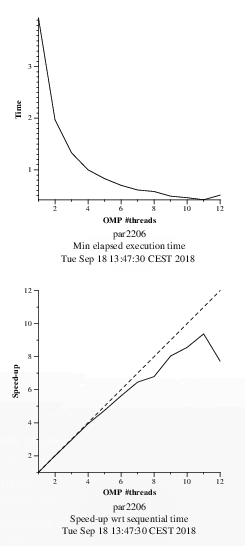
\includegraphics[width=0.45\linewidth, height=0.6\linewidth]{strongPI.png}
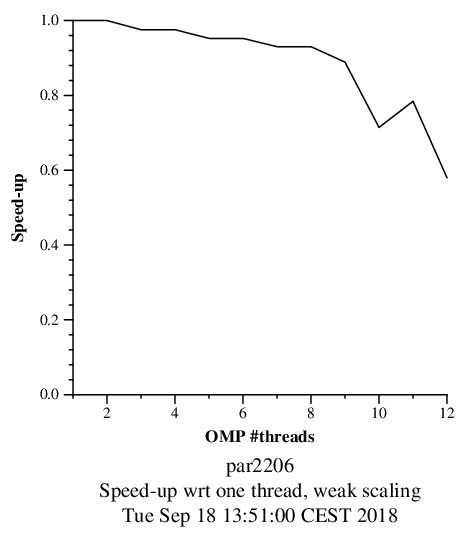
\includegraphics[width=0.45\linewidth, height=0.6\linewidth]{weakPI.png}
\end{wrapfigure}

When we refer to strong scalability we address to the increase of speedup when we increase the number of resources with a fixed problem size\newline
On the other hand, with weak scalability we measure the performance when the problem size is increased proportional to the number of resources.\newline
In the following figure we can observe that in strong scalability time decreases with more threads and in weak it decreases due to overheads (the ideal situation would be an straight line).\newline \newline \newline

\section*{Analysis of task decompositions for 3DFFT}
This table shows the increment of parallelism between each version due to the bigger granularity. 
\begin{center}
    \begin{tabular}{ | l || l | l | 1 |}
    \hline
     Version & $T_1$ & $T_\infty$ & Parallelism \\ \hhline{|=|=|=|=|}
     Seq & 0,64 s & 0.64 s & 1 \\ \hline
     v1  & 0.64 s & 0.64 s & 1 \\ \hline
     v2  & 0.64 s & 0.36 s & 1.78 \\ \hline
     v3  & 0.64 s & 0.15 s & 4.27 \\ \hline
     v4  & 0.64 s & 0.064 s & 10.67 \\ \hline
     v5  & 0.64 s & 0.008 s & 80 \\ \hline
    \end{tabular}
    
\end{center}
The granularity of V4 is on the 'k' loop, which is the outer one. In the V5 there is more granularity since it is at 'j' level as we can see in this sample of code:
\begin{lstlisting}
    for (k=0; k<N; k++) {
     for (j=0; j<N; j++) {
    tareador_start_task("transpose_zx_planes_loop_j");
       for (i=0; i<N; i++)
       {
         in_fftw[i][j][k][0] = tmp_fftw[k][j][i][0];
         in_fftw[i][j][k][1] = tmp_fftw[k][j][i][1];
       }
     tareador_end_task("transpose_zx_planes_loop_j");

     }
}
\end{lstlisting}
In this two graphics we can see the impact of the granularity in the scalability. V4's granularity limits the time improvement at 8 threads. Instead, V5 continues improving with more threads. \newline \newline
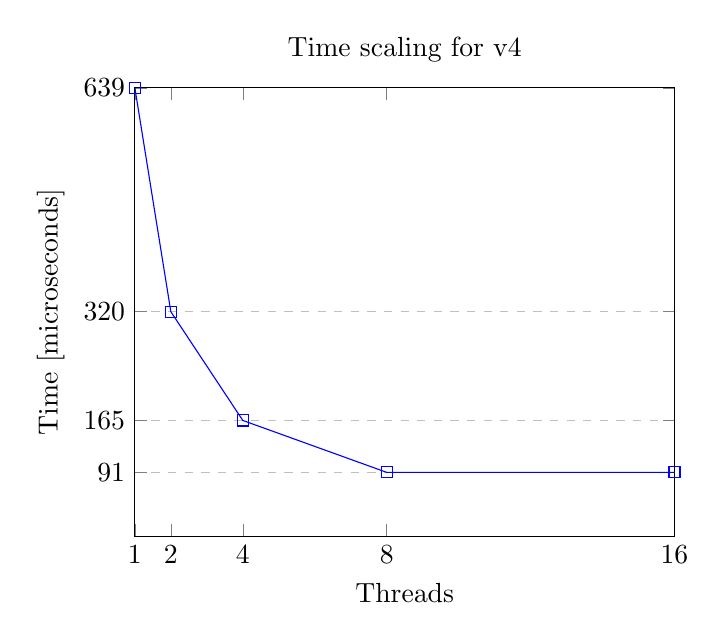
\begin{tikzpicture}
\begin{axis}[
    title={Time scaling for v4},
    xlabel={Threads },
    ylabel={Time [microseconds]},
    xmin=1, xmax=16,
    ymin=0, ymax=639,
    xtick={1,2,4,8,16},
    ytick={639,320,165,91},
    legend pos=north west,
    ymajorgrids=true,
    grid style=dashed,
]
 
\addplot[
    color=blue,
    mark=square,
    ]
    coordinates {
    (1,639)(2,320)(4,165)(8,91)(16,91)
    };
    
 
\end{axis}
\end{tikzpicture}
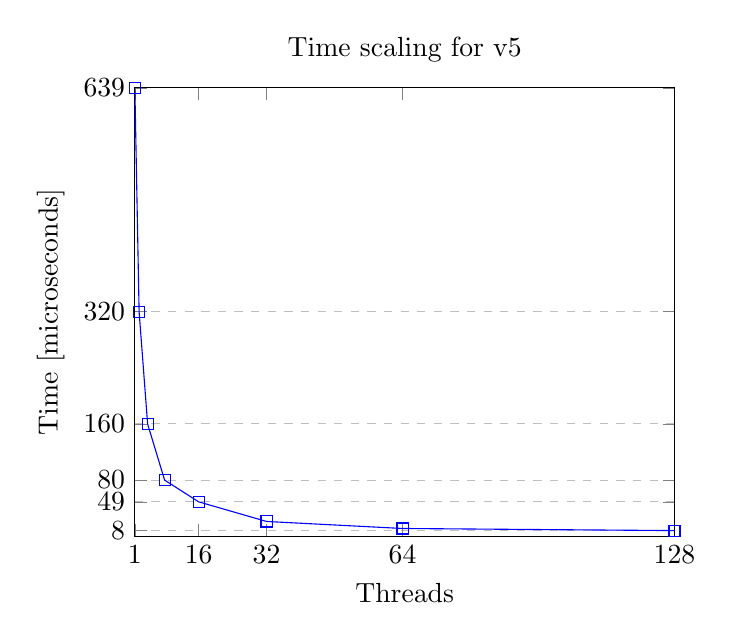
\begin{tikzpicture}
\begin{axis}[
    title={Time scaling for v5},
    xlabel={Threads },
    ylabel={Time [microseconds]},
    xmin=1, xmax=128,
    ymin=0, ymax=639,
    xtick={1,16,32,64,128},
    ytick={639,320,160,80,49,8},
    legend pos=north west,
    ymajorgrids=true,
    grid style=dashed,
]
 
\addplot[
    color=blue,
    mark=square,
    ]
    coordinates {
    (1,639)(2,320)(4,160)(8,80)(16,49)(32,21)(64,11)(128,8)
    };
\end{axis}
\end{tikzpicture}
\section*{Understanding the parallel execution of 3DFFT}
\begin{center}
    \begin{tabular}{ | 1 || l | l || l | 1 | 1 |}
    \hline
     Version & $\Phi$ & $S_\infty$ & $T_1$ & $T_8$ & $S_8$ \\ \hhline{|=|=|=|=|=|=|}
     Initial         & 0.54 & 2.15 & 2.89 s & 1.41 s & 2.05 \\ \hline
     Improved $\Phi$ & 0.89 & 9.09 & 2.30 s & 0.81 s & 3.52 \\ \hline
     Improved parallel overheads & 0.88 & 8.33 & 2.20 s & 0.80 s & 2.75 \\ \hline
     improved work-distribution overheads & 0.87  & 7.74 & 2.19 s & 0.44 s & 4.97 \\ \hline
    \end{tabular}
\end{center}
\subsection*{Improved $\Phi$}
In the improved version we added the parallelization instrumentation to the init complex grid routine.
\csvautotabular{improved8.csv}
\subsection*{Improved parallel overheads}
For the sake of reducing overheads we moved the threads creation outside the loops so we don't create them each 'k' iteration.We can observe that the time of the threads not being created is increased and also the running times are lowered.\newline
\csvautotabular{overheads8.csv}
\subsection*{Improved work-distribution overheads}
On this final version we moved the work-distribution pragma outside the loops, so the overhead of distributing the work each loop is removed. In the table we can observe that the time the threads were running is lowered and that the value of synchronisation is the same,with the time not being created has increased.\newline\newline
\csvautotabular{workdist8.csv}
\newpage
\subsection*{Strong scallability plots}
You can take a look at strong scallability plots to confirm that with each optimisation we obtain better results. 
\begin{figure}[htbp]
    \centering
    \begin{subfigure}[b]{0.35\textwidth}                                        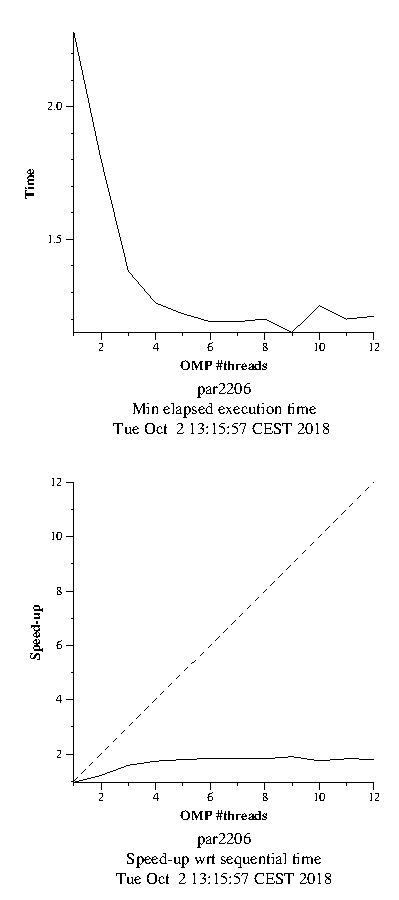
\includegraphics[width=\textwidth]{stronginitial.png}
        \caption{Initial version}
    \end{subfigure}
    \begin{subfigure}[b]{0.35\textwidth}
        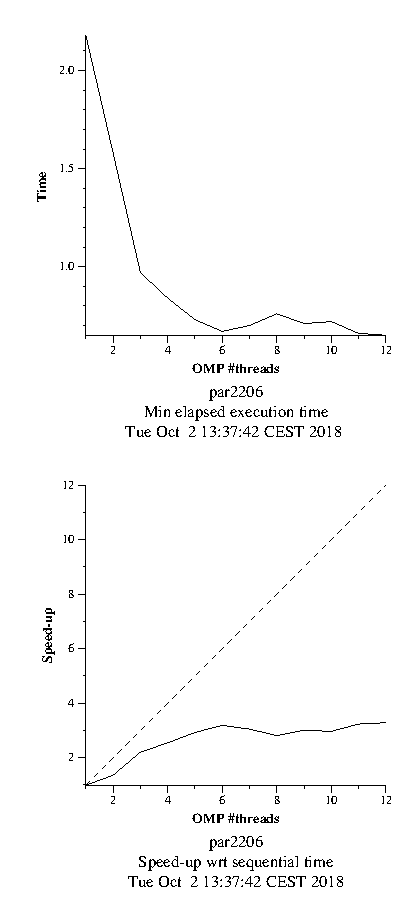
\includegraphics[width=\textwidth]{strongimproved1.png}
        \caption{Improved $\Phi$}
    \end{subfigure}
\end{figure}
\newpage
\begin{figure}[htbp]
    \centering
    \begin{subfigure}[b]{0.35\textwidth}                                        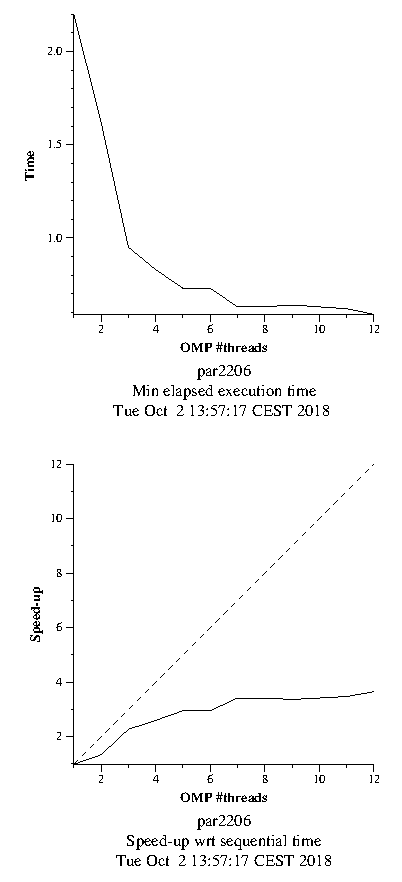
\includegraphics[width=\textwidth]{strongoverhead.png}
        \caption{Improved parallel overheads}
    \end{subfigure}
    \begin{subfigure}[b]{0.35\textwidth}
        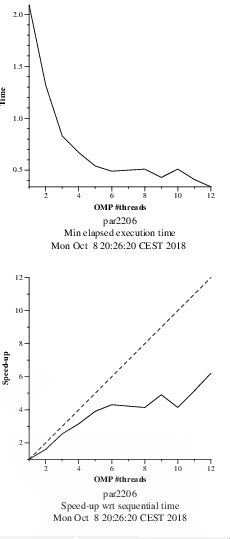
\includegraphics[width=\textwidth]{strongWorkDist.png}
        \caption{Improved work-distribution overheads}
    \end{subfigure}
\end{figure}

\end{document}
